This project is analysis for Korean Herald Dataset by using different two methods. The first task is Issue Trend Analysis. The goal of the task is to find most important, meaningful top 10 topics among those data set. The second task is Issue Tracking which is to find events based on a specific issue from Issue Trend Analysis and give details of the event. The specific tasks are divided into On-issue Event Tracking and Related-issue Tracking. For solving those tasks, Team5 use the process as follows.
\begin{figure*}[htp]
    \centering            
    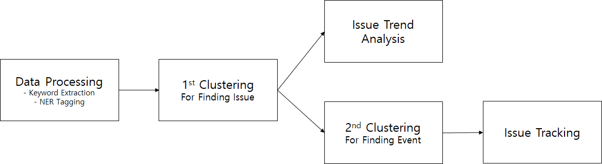
\includegraphics[width=\textwidth]{01_introduction.png} 
    \caption{The process of project} 
    \label{fig:introduction} 
\end{figure*}\\
In Data Processing step, find keywords and Named Entity of News documents and those results will be used in whole process of project.The First Clustering is generating clusters based on the information from previous step. Next step is Issue Trend Analysis from the results of First Clustering. Issue Trends are ranked by number of documents in a cluster. The process of Second Clustering is for searching events in Issues. In this step, we will use the information of Data Processing and the text data which are not used yet. Finally, Issue tracking will be done by using the result of Second Clustering.